% !TEX program = xelatex
% 编译方式：xelatex milestone_report.tex （需支持中文的 XeLaTeX + ctex 宏包）
\documentclass[11pt]{ctexart}

\usepackage{graphicx} 
\usepackage{amsmath}
\usepackage{amssymb}
\usepackage{booktabs}
\usepackage{tabularx}
\usepackage{geometry}
\usepackage{xcolor}
\usepackage{enumitem}
\usepackage{hyperref}
\hypersetup{colorlinks=true, linkcolor=blue, urlcolor=blue}

\geometry{a4paper, margin=2.5cm}

% 行内代码样式
\newcommand{\code}[1]{\texttt{#1}}

% 引用框（用于"手算示例 / 关键点"等旁注）
\newenvironment{note}
  {\begin{quote}\itshape\small\color{black!75}}
  {\end{quote}}

\title{\textbf{几何计算前沿 Milestone}\\[4pt]
       \large 选题：3D 分形自回归模型（FractalOctGen）}
\author{李睿钦，董彦嘉，王宝骥}
\date{\today}

\begin{document}
\maketitle

%==================================================================
\section{选题背景}

Kaiming He 等人提出的 \textbf{分形生成模型（Fractal Generative Model, FractalGen）} 为自回归生成提供了一种新思路：把“逐像素自回归”这一计算量极大的过程，\textbf{递归地分解为多个层级、局部化的小自回归问题}。每一层只负责在一个较粗的网格上预测下一层更精细的若干子单元，再把每个子单元递归交给同构的下一级生成器。

本次作业的目标是：\textbf{将 FractalGen 从二维图像生成拓展到三维形状生成}。三维数据天然具有层级空间结构——把单位立方体递归地八等分，每个节点对应一个空间子区域，是否继续细分取决于该区域是否包含物体表面。

我们使用 ShapeNet \textbf{airplane} 类（synset \code{02691156}，共 \textbf{4045} 个网格模型）作为验证数据。飞机类结构有明显的整体轮廓和精细局部，适合检验框架。

%==================================================================
\section{方法原理}

%------------------------------------------------------------------
\subsection{数据表示：从网格到八叉树张量}

\textbf{(a) 建树。} 给定一个网格：在表面均匀采样 $P=10^5$ 个点 $\{p_i\}$ 及法向 $\{n_i\}$；做归一化
\[
c=\tfrac{1}{2}(\max_i p_i+\min_i p_i),\quad
s=\max_i\|p_i-c\|_\infty,\quad
\hat p_i=\frac{p_i-c}{s}\cdot 0.9 .
\]
于是点云落在 $[-0.9,0.9]^3$。从根立方体开始递归八等分：\textbf{一个节点只要其内部含有采样点，就继续细分}，直到深度 7。

\textbf{(b) 提取张量。} 对每个深度 $d$（$2\le d\le 6$），从树里取以下信息：

\begin{enumerate}[leftmargin=*]
\item \textbf{分裂标签} $\mathrm{split}_d\in\{0,1\}^{N_d}$：第 $i$ 个节点是否有孩子，$1$ = 该 cell 含表面、要继续细分；$0$ = 空兄弟节点。
\item \textbf{坐标} $\mathrm{xyz}_d\in[0,1]^{N_d\times 3}$：把节点的 Morton 码解码成整数格坐标 $(x,y,z)\in\{0,\dots,2^d-1\}^3$，再归一化
  \[\mathrm{xyz}_d[i]=\frac{(x_i,y_i,z_i)}{2^d-1}\in[0,1]^3.\]
\item \textbf{父索引} $\mathrm{parent\_idx}_d\in\{0,\dots,N_{d-1}-1\}^{N_d}$：ocnn 保证一个分裂节点的 8 个孩子在下一层是\textbf{连续的 8 个}。若 depth-$(d{-}1)$ 第 $i$ 个节点的 \code{children[i]=c}，则 depth-$d$ 的第 $c,c{+}1,\dots,c{+}7$ 个节点的父索引都为 $i$。
\end{enumerate}

节点在每层按 \textbf{z-order（Morton 码）} 排列，因此同一父节点的 8 个孩子是连续 8-块，序列上相邻的节点在三维空间中也大概率相邻。

%------------------------------------------------------------------
\subsection{计算细节}

设输入是某层 $N$ 个节点的特征矩阵 $X\in\mathbb{R}^{N\times D}$（忽略 batch 维）。

\paragraph{(1) 三维正弦位置编码 $\mathrm{PE}(\mathrm{xyz})$。}
取频率个数 $F=\lfloor D/6\rfloor$，指数在 $[0,\,\code{OCTREE\_DEPTH}{-}1]=[0,6]$ 上等距取 $F$ 个：
\[
e_k=\frac{6k}{F-1}\ (k=0..F{-}1),\qquad f_k=2^{e_k}\cdot\pi .
\]
对坐标 $(x,y,z)$，每个轴各做 $\sin,\cos$，拼成长度 $6F$ 的向量（不足 $D$ 补零）：
\[
\mathrm{PE}=\big[\sin(x f_k),\cos(x f_k),\ \sin(y f_k),\cos(y f_k),\ \sin(z f_k),\cos(z f_k)\big]_{k=0}^{F-1}.
\]

最高频 $f_{F-1}=2^6\pi=64\pi$，最细一级相邻格间距为 $1/63$，相位差约 $64\pi/63\approx\pi$，刚好能区分相邻格。

\paragraph{(2) 因果自注意力。}
先 LayerNorm 得 $\tilde X$，线性映射出 Q/K/V（无偏置），分 $H$ 头，每头 $d_h=64$：
\[
A=\mathrm{softmax}\!\Big(\frac{QK^\top}{\sqrt{d_h}}+M\Big),\qquad
\mathrm{Out}=A\,V,
\]
其中\textbf{因果掩码} $M_{ij}=-\infty$ 当 $j>i$，否则 $0$，保证第 $i$ 个节点只能看自己和前面的节点。多头拼接后过输出投影 $W_o$，再残差相加。

\paragraph{(3) SwiGLU 前馈。}
设隐藏宽度 $h=4D$：
\[
[a,b]=\mathrm{LN}(x)\,W_1\ ,\qquad
\mathrm{FFN}(x)=\big(\mathrm{SiLU}(a)\odot b\big)W_2,\qquad \mathrm{SiLU}(t)=t\,\sigma(t),
\]
再残差相加。一个 Transformer block $=$ 注意力残差 $+$ SwiGLU 残差。

\paragraph{(4) 窗口化双向注意力。}
把 $N$ 个节点按顺序切成长度 $W=64$ 的窗口（不足补零并屏蔽），\textbf{在每个窗口内做无因果掩码的双向注意力}（公式同 (2) 但 $M=0$）。复杂度 $O(N\cdot W\cdot D)$，远小于全局的 $O(N^2 D)$。让同一父节点的 8 个孩子、以及 z-order 相邻的邻居互相“看到”，协调表面，但\textbf{不引入任何前后顺序}。

%------------------------------------------------------------------
\subsection{两类层级生成器的前向}

\paragraph{(A) 自回归层 OctAR（用于 $d=2,3$）。}
输入：该层标签 $\mathrm{split}_d\in\{0,1\}^N$、坐标 $\mathrm{xyz}_d$、父条件 $C^{\mathrm{par}}\in\mathbb{R}^{N\times D}$。
\begin{enumerate}[leftmargin=*]
\item \textbf{右移一位}（teacher forcing）：在序列开头插入 BOS 记号（标签值 2），丢掉最后一个：
  $\mathrm{in}=[2,\ \mathrm{split}_d[0],\dots,\mathrm{split}_d[N{-}2]]$。这样预测第 $i$ 个标签时，输入只含第 $0..i{-}1$ 个真值，不会偷看答案。
\item \textbf{三路相加得节点嵌入}：
  \[X = \underbrace{\mathrm{Emb}(\mathrm{in})}_{\text{标签嵌入}} + \underbrace{\mathrm{PE}(\mathrm{xyz}_d)W_{\mathrm{pos}}}_{\text{位置}} + \underbrace{C^{\mathrm{par}}W_{\mathrm{cond}}}_{\text{父条件}} \in\mathbb{R}^{N\times D}.\]
\item 过 $L$ 个\textbf{因果} Transformer block（\code{base}：$d{=}2$ 用 14 层，$d{=}3$ 用 10 层），最后 LayerNorm。
\item \textbf{两个输出头}：
  \[z_i=\mathrm{split\_head}(X_i)\in\mathbb{R}\ \text{(分裂 logit)},\qquad
  C^{\mathrm{out}}_i=\mathrm{cond\_out}(X_i)\in\mathbb{R}^{D}\ \text{(给子层的条件)}.\]
\end{enumerate}

\paragraph{(B) 并行占据层 OccupancyMLP（用于 $d=4,5,6$）。}
输入：坐标 $\mathrm{xyz}_d$、父条件 $C^{\mathrm{par}}$。
\begin{enumerate}[leftmargin=*]
\item 位置特征 $g=\mathrm{PE}(\mathrm{xyz}_d)\,W_{\mathrm{pos}}\in\mathbb{R}^{N\times D}$。
\item 拼接父条件与位置，过 MLP trunk（首层 $\mathbb{R}^{2D}\!\to\!\mathbb{R}^{D}$，其后若干层 $\mathbb{R}^{D}\!\to\!\mathbb{R}^{D}$，激活 SiLU）：
  \[h=\mathrm{trunk}\big([\,C^{\mathrm{par}}\,\|\,g\,]\big)\in\mathbb{R}^{N\times D}.\]
\item 过若干\textbf{窗口化双向注意力} block（同层协调）：$h\leftarrow \mathrm{WinBlock}(h)$。
\item 两个输出头（同 OctAR）：分裂 logit $z_i$ 与子条件 $C^{\mathrm{out}}_i$。
\end{enumerate}

\paragraph{(C) 条件级联。}
第 $k$ 层输出每个节点的 $C^{\mathrm{out}}$。第 $k{+}1$ 层每个子节点 $j$ 的父条件，就是按父索引去取对应父节点的输出：
\[
C^{\mathrm{par}}_{(k+1)}[j]=C^{\mathrm{out}}_{(k)}\big[\mathrm{parent\_idx}[j]\big].
\]
最顶层（$d=2$）没有父层，父条件用一个可学习的\textbf{类别嵌入向量}（单类飞机即固定一个向量）。信息从 $d{=}2$ 自顶向下流到 $d{=}6$，\textbf{每级结构同构、权重独立，靠条件向量相互联系}。

%------------------------------------------------------------------
\subsection{训练过程}

训练是\textbf{广度优先}的，对一个样本（去掉 batch 维）：
\begin{enumerate}[leftmargin=*]
\item $C^{\mathrm{par}}\leftarrow$ 类别嵌入（广播到 $d{=}2$ 的 64 个节点）。
\item \textbf{for $d=2,3$（OctAR）}：用 2.3(A) 算出 logits $z^{(d)}$ 与 $C^{\mathrm{out}}$；若 $d=3$，先用 2.3(C) 从上一层 gather 父条件。
\item \textbf{for $d=4,5,6$（OccupancyMLP）}：用 2.3(C) gather 父条件，再用 2.3(B) 算 logits 与 $C^{\mathrm{out}}$。
\item \textbf{每层的损失}（带正样本权重的二值交叉熵，只在有效节点上算）：
  \[
  w_d=\mathrm{clip}\!\Big(\frac{\#\{y=0\}}{\#\{y=1\}},\,0.5,\,10\Big),\quad
  \mathcal L_d=\frac1{N_d}\sum_{i}\Big[-w_d\,y_i\log\sigma(z_i)-(1-y_i)\log\big(1-\sigma(z_i)\big)\Big],
  \]
  其中 $y_i=\mathrm{split}_d[i]$。$w_d$ 逐 batch、逐层动态估计，用来对抗“空节点远多于表面节点”的类别不均衡。
\item \textbf{总损失} $\mathcal L=\sum_{d=2}^{6}\mathcal L_d$，对它反向传播、AdamW 更新。
\end{enumerate}

%------------------------------------------------------------------
\subsection{生成过程}

生成是\textbf{深度优先}的，且因为各形状的树结构不同，逐个形状生成。

\paragraph{depth-2 的 64 个固定节点。}
$d{=}2$ 全展开，坐标固定为 $4\times4\times4$ 网格：对 Morton 码 $\mathrm{key}=0..63$ 解码出整数坐标后除以 3。父条件 = 类别嵌入。

\paragraph{自回归生成 depth-2 的分裂标签（64 步循环）。}
逐节点调用 OctAR：第 $t$ 步把已生成的 $t$ 个标签（前面加 BOS）+ 前 $t{+}1$ 个坐标/父条件喂进去，取最后位置的 logit $z_t$，按温度采样，同时记录该位置的 $C^{\mathrm{out}}_t$。循环 64 次得到 $\mathrm{split}_2$ 与 64 个 $C^{\mathrm{out}}$。（温度 $\tau=$\code{temperature\_l0}。）

\paragraph{自回归生成 depth-3。}
\begin{itemize}[leftmargin=*]
\item \textbf{展开}：找出 $\mathrm{split}_2=1$ 的父节点，每个生成 8 个孩子。孩子坐标用 2.1(c) 的公式：父整数坐标 $=\mathrm{xyz}\times(2^2{-}1)$，孩子整数坐标 $=2\times$父$+\{0,1\}^3$，再除以 $2^3{-}1=7$。孩子的父条件 = 该父节点的 $C^{\mathrm{out}}$（每个父复制 8 份）。
\item \textbf{自回归采样}：把这 $N_3$ 个孩子按顺序，像第 1 步一样逐个跑 OctAR（温度 \code{temperature\_l1}），得到 $\mathrm{split}_3$ 与每个孩子的 $C^{\mathrm{out}}$。
\end{itemize}

\paragraph{并行生成 depth-4、5、6（级联）。} 对 $d=4,5,6$ 依次：
\begin{itemize}[leftmargin=*]
\item \textbf{展开}：找出上一层 $\mathrm{split}=1$ 的父节点，按公式生成 8 个孩子坐标（公式同上，父整数坐标用 $2^{d-1}{-}1$、孩子除以 $2^{d}{-}1$），父条件复制 8 份。
\item \textbf{并行预测}：把所有孩子一次性喂进 OccupancyMLP（含窗口注意力），得到每个孩子的 logit $z_i$ 与 $C^{\mathrm{out}}$。最后采样占据。
\end{itemize}

\paragraph{体素化。}
取最细层 $d{=}6$ 中 $\mathrm{split}_6=1$ 的节点，把归一化坐标还原成 $64^3$ 网格的整数索引并置 1：
\[
\mathrm{idx}=\mathrm{round}\big(\mathrm{xyz}_6\times(2^6-1)\big)\in\{0,\dots,63\}^3,\qquad \mathrm{grid}[\mathrm{idx}]=\mathrm{True}.
\]

\paragraph{薄壳 $\to$ 实体 $\to$ 网格。}
上一步得到的是一层薄壳，直接 Marching Cubes 会出现双壁和孔洞，故先后处理：\textbf{形态学闭运算}$\to$ \textbf{填充内部}$\to$ \textbf{保留最大连通分量}；再 \textbf{Marching Cubes}$\to$ \textbf{Taubin 平滑}$\to$ 导出 OBJ。

%==================================================================
\section{作业进展}

\subsection{已完成}
数据管线、模型实现、训练框架、生成与可视化、端到端验证均已实现。

\subsection{当前效果}
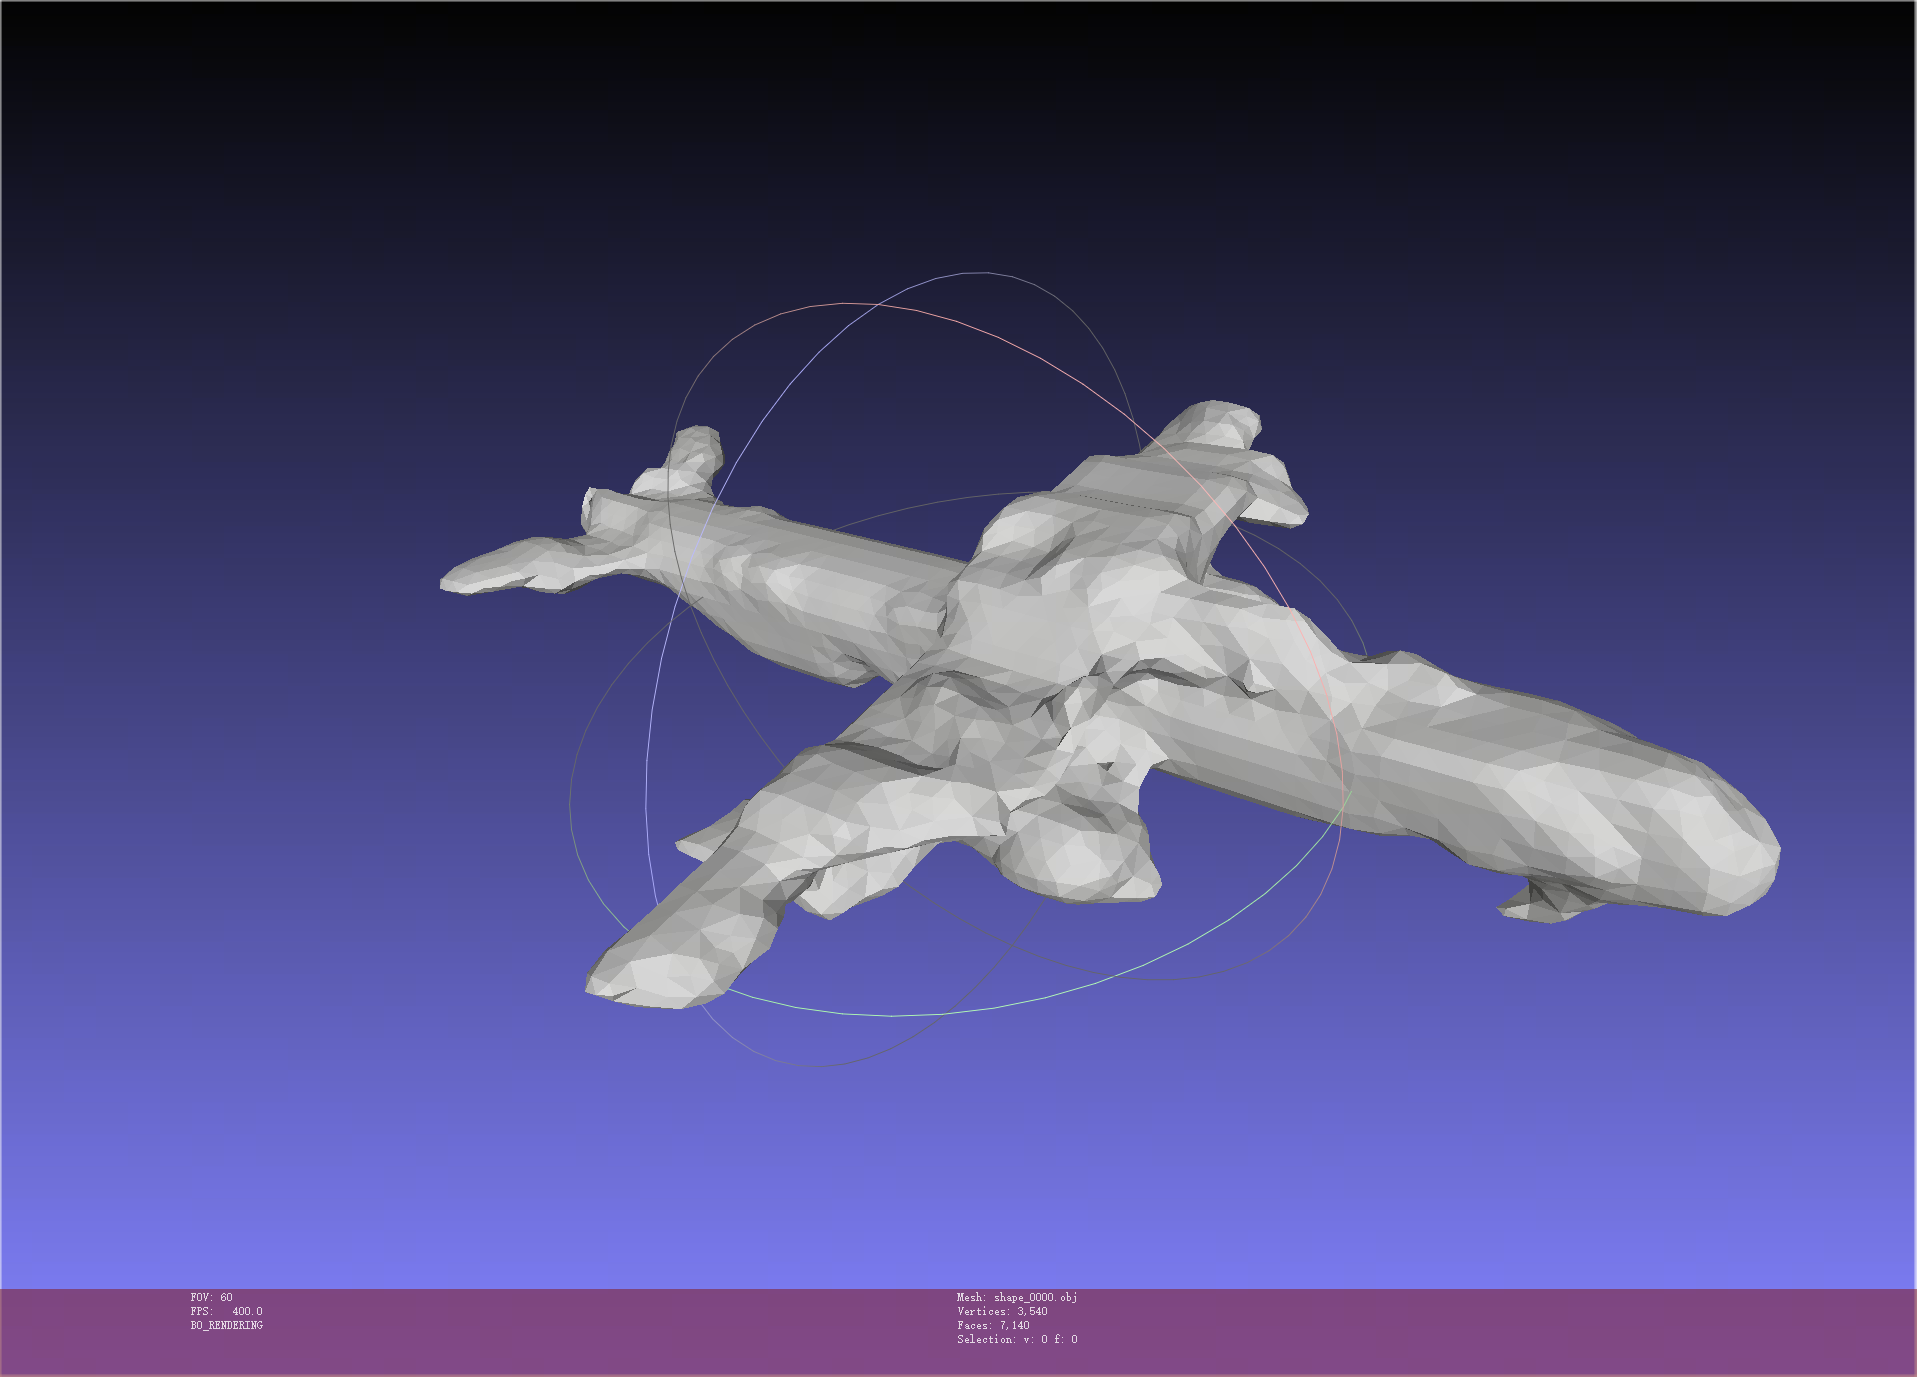
\includegraphics[width=0.8\textwidth]{image.png}

整体轮廓正确，多数样本能看出是飞机。但表面仍\textbf{粗糙}，局部有起伏；少数样本整体结构仍不够像飞机。可能原因包括：
(1) 表示为\textbf{硬二值占据 + 薄壳}，先天不利于光滑水密表面；(2) 细层并行 + 局部注意力只能局部协调，缺乏全局精修；(3) 训练可能尚未在最细层（\code{loss\_d6}）充分收敛。

%==================================================================
\section{改进方向}

\begin{enumerate}[leftmargin=*]
\item \textbf{连续场表示}：把最细层从二值占据换成 \textbf{SDF/TSDF 或连续占据概率}，在连续标量场上提面，天然光滑、水密。
\item \textbf{更深的自回归层 / 更强条件}：把自回归层延伸到 depth-4，或在细层引入跨父节点的稀疏 3D 卷积，进一步增强全局一致性。
\item \textbf{更充分的训练与调参}：确认 \code{loss\_d6} 收敛；调节 \code{pos\_weight}、模型规模与训练时长。
\end{enumerate}

\end{document}
